\documentclass[a4paper, 12pt]{article}
\usepackage[utf8]{inputenc}
\usepackage[english]{babel}
\usepackage{graphicx}
\usepackage{hyperref}
\usepackage[a4paper]{geometry}
%\usepackage[left=1cm,right=2cm,vmargin=2.5cm,footnotesep=0.5cm]{geometry}
\usepackage{amssymb,amsmath,amsthm}
\DeclareMathOperator*{\E}{\mathbb{E}}
\DeclareMathOperator*{\Var}{\text{Var}}
\renewcommand*{\P}{\mathbb{P}}
\newtheorem{theorem}{Theorem}
\newtheorem{lemma}{Lemma}

\hypersetup{
    colorlinks=true,
    linkcolor=blue,
    filecolor=magenta,      
    urlcolor=cyan,
    pdftitle={Sharelatex Example},
    bookmarks=true,
    pdfpagemode=FullScreen
}

  
\begin{document} 

\begin{titlepage}
	\centering
	{\scshape\LARGE Ozonmasters \par}
	\vspace{1cm}
	{\scshape\Large Statistics \par}
	\vspace{1.5cm}
	{\huge\bfseries Home work \par}
	\vspace{2cm}
	{\Large\itshape Kozhemyak Vitaly \par}
	\vfill

% Bottom of the page
	{\large \today\par}
\end{titlepage}
  
\tableofcontents

\newpage
 
In this article we denote $X_1, \ldots X_n$ as a sequence of i.i.d random variables and $x_1, \ldots, x_n$ as a sample.
\section{Task 1}
\subsection{Theoretical solution} Let $(1, 2, 3)$ be the events like "rock, scissors, paper". Consider $\eta, \eta_1, \eta_2 \sim P$ on $[0, 1]$ and random variables 
$$
X = 
\begin{cases}
1, & p, \\
2, & q, \\
3, & 1 - p - q,
\end{cases}
$$
$$
Y = 
\begin{cases}
1, & \eta_{(1)}, \\
2, & \eta_{(2)} - \eta_{(1)}, \\
3, & 1 - \eta_{(2)}.
\end{cases}
$$
$$
\P (1st \ win) = \P(\{ X=1, Y=2\} \cup \{ X=2, Y=3 \} \cup \{ X=3, Y=1 \}) = 
$$
$$
 = \P(X=1) \P(Y=2) + \P(X=2) \P(Y=3) + \P(X=3) \P(Y=1) = 
$$
\begin{eqnarray*}
= p \int \limits_0^1 \P(Y=2 | \eta_{(2)} - \eta_{(1)} = x) f_{\eta_{(2)} - \eta_{(1)}}(x) dx + \\
+ q \int \limits_0^1 \P(Y=3 | 1 - \eta_{(2)} = x) f_{1-\eta_{(2)}}(x) dx + \\
+ (1 - p - q) \int \limits_0^1 \P(Y=1 | \eta_{(1)} = x) f_{\eta_{(1)}}(x) dx = 
\end{eqnarray*}
$$
= p\E [\eta_{(2)} - \eta_{(1)}] + q \E [1 - \eta_{(2)}] + (1 - p - q) \E[\eta_{(1)}] = 
$$
\begin{equation}
\label{expected_value}
= (\E [\eta_{(2)}] - 2\E[\eta_{(1)}] ) p  + (1 - \E [\eta_{(2)}] - \E[\eta_{(1)}]) q  + \E[\eta_{(1)}].
\end{equation}

\begin{lemma}
Consider $X_1, \ldots X_n $ as a sequence of i.i.d random variables with some distribution $P.$ Then
$$
F_{X_{(n)}}(x) = F_{X}^n(x), 
$$
$$
F_{X_{(1)}}(x) = 1 - (1 - F_{X}(x))^n
$$
where $X$ has the same distribution $P$ on $[0, 1].$
\end{lemma}
\begin{proof} Let's deduce the \textbf{distribution of maximum}
$$
F_{X_{(n)}}(x) = \P(X_{(n)} \leqslant x) = \P (X_{1} \leqslant x, \ldots, X_{n} \leqslant x) =
$$
$$
 =\prod \limits_{i=1}^n \P(X_{i} \leqslant x) = F_{X}^n(x), 
$$
and \textbf{distribution of minimum} 
$$
F_{X_{(1)}}(x) = \P(X_{(1)} \leqslant x) = 1 - \P(X_{(1)} > x) = \P (X_{1} > x, \ldots, X_{n} > x) = 
$$
$$
 = 1 - \prod \limits_{i=1}^n \P(X_{i} > x) = 1 - \prod \limits_{i=1}^n(1 - \P(X_{i} \leqslant x)) = 1 - (1 - F_{X}(x))^n.
$$
\end{proof}
\noindent Now we can calculate the expected values: 
$$
\E[\eta_{(1)}] = \int \limits_{-\infty}^{+\infty} x f_{\eta_{(1)}}(x) dx = 2\int \limits_{-\infty}^{+\infty} x (1 - F_X(x)) f_{X}(x) dx = 2 (\E[X] - \E [X F_X(X)]), 
$$
$$
\E[\eta_{(2)}] = \int \limits_{-\infty}^{+\infty} x f_{\eta_{(2)}}(x) dx = 2 \int \limits_{-\infty}^{+\infty} x  F_X(x) f_{X}(x) dx = 2 \E [X F_X(X)].
$$
Remember the last equation in \eqref{expected_value} and make the substitution of expected values we have found above
$$
\P (1st \ win) = (6 \E[X F_X(X)] - 4 \E[X]) p + (1 - 2 \E[X]) q + 2 (\E[X] - \E [X F_X(X)]).
$$
We want to maximize $\P (1st \ win)$ in $p, q$, so consider the next linear optimization problem:
$$
\begin{cases}
\alpha p + \beta q \rightarrow \max \limits_{p, q}, \\
p + q \leqslant 1, \\
p \geqslant 0, q \geqslant 0.
\end{cases}
$$
The solution of this problem is
\begin{enumerate}
	\item $\alpha < \beta \Rightarrow q = 1, p = 0;$
	\item $\alpha > \beta \Rightarrow q = 0, p = 1;$
	\item $\alpha = \beta \geqslant 0 \Rightarrow p + q = 1;$
	\item $\alpha = \beta < 0 \Rightarrow p = q = 0;$
	\item $\beta < \alpha = 0 \Rightarrow q = 0, p = [0, 1];$
	\item $\alpha < \beta = 0 \Rightarrow q = [0, 1], p = 0.$
\end{enumerate}
So, put $\alpha = 6 \E[X F_X(X)] - 4 \E[X], \beta = 1 - 2 \E[X].$ If the players have played $n$ rounds before then we can estimate 
$$
\E[X] = \dfrac{1}{n} \sum \limits_{i=1}^n x_i.
$$
Split last $n$ games as follows $\{1, \ldots m \} + \{ m+1, \ldots, n \}.$ Then
$$
F_X(x) \approx F_n(x) = \dfrac{1}{m} \sum \limits_{j=1}^m \mathbb{I}[x_j \leqslant x],
$$
$$
\E [X F_X(X)] = \dfrac{1}{n - m} \sum \limits_{i = m+1}^n x_i F_n(x_i).
$$
\subsection{Numerical solution}
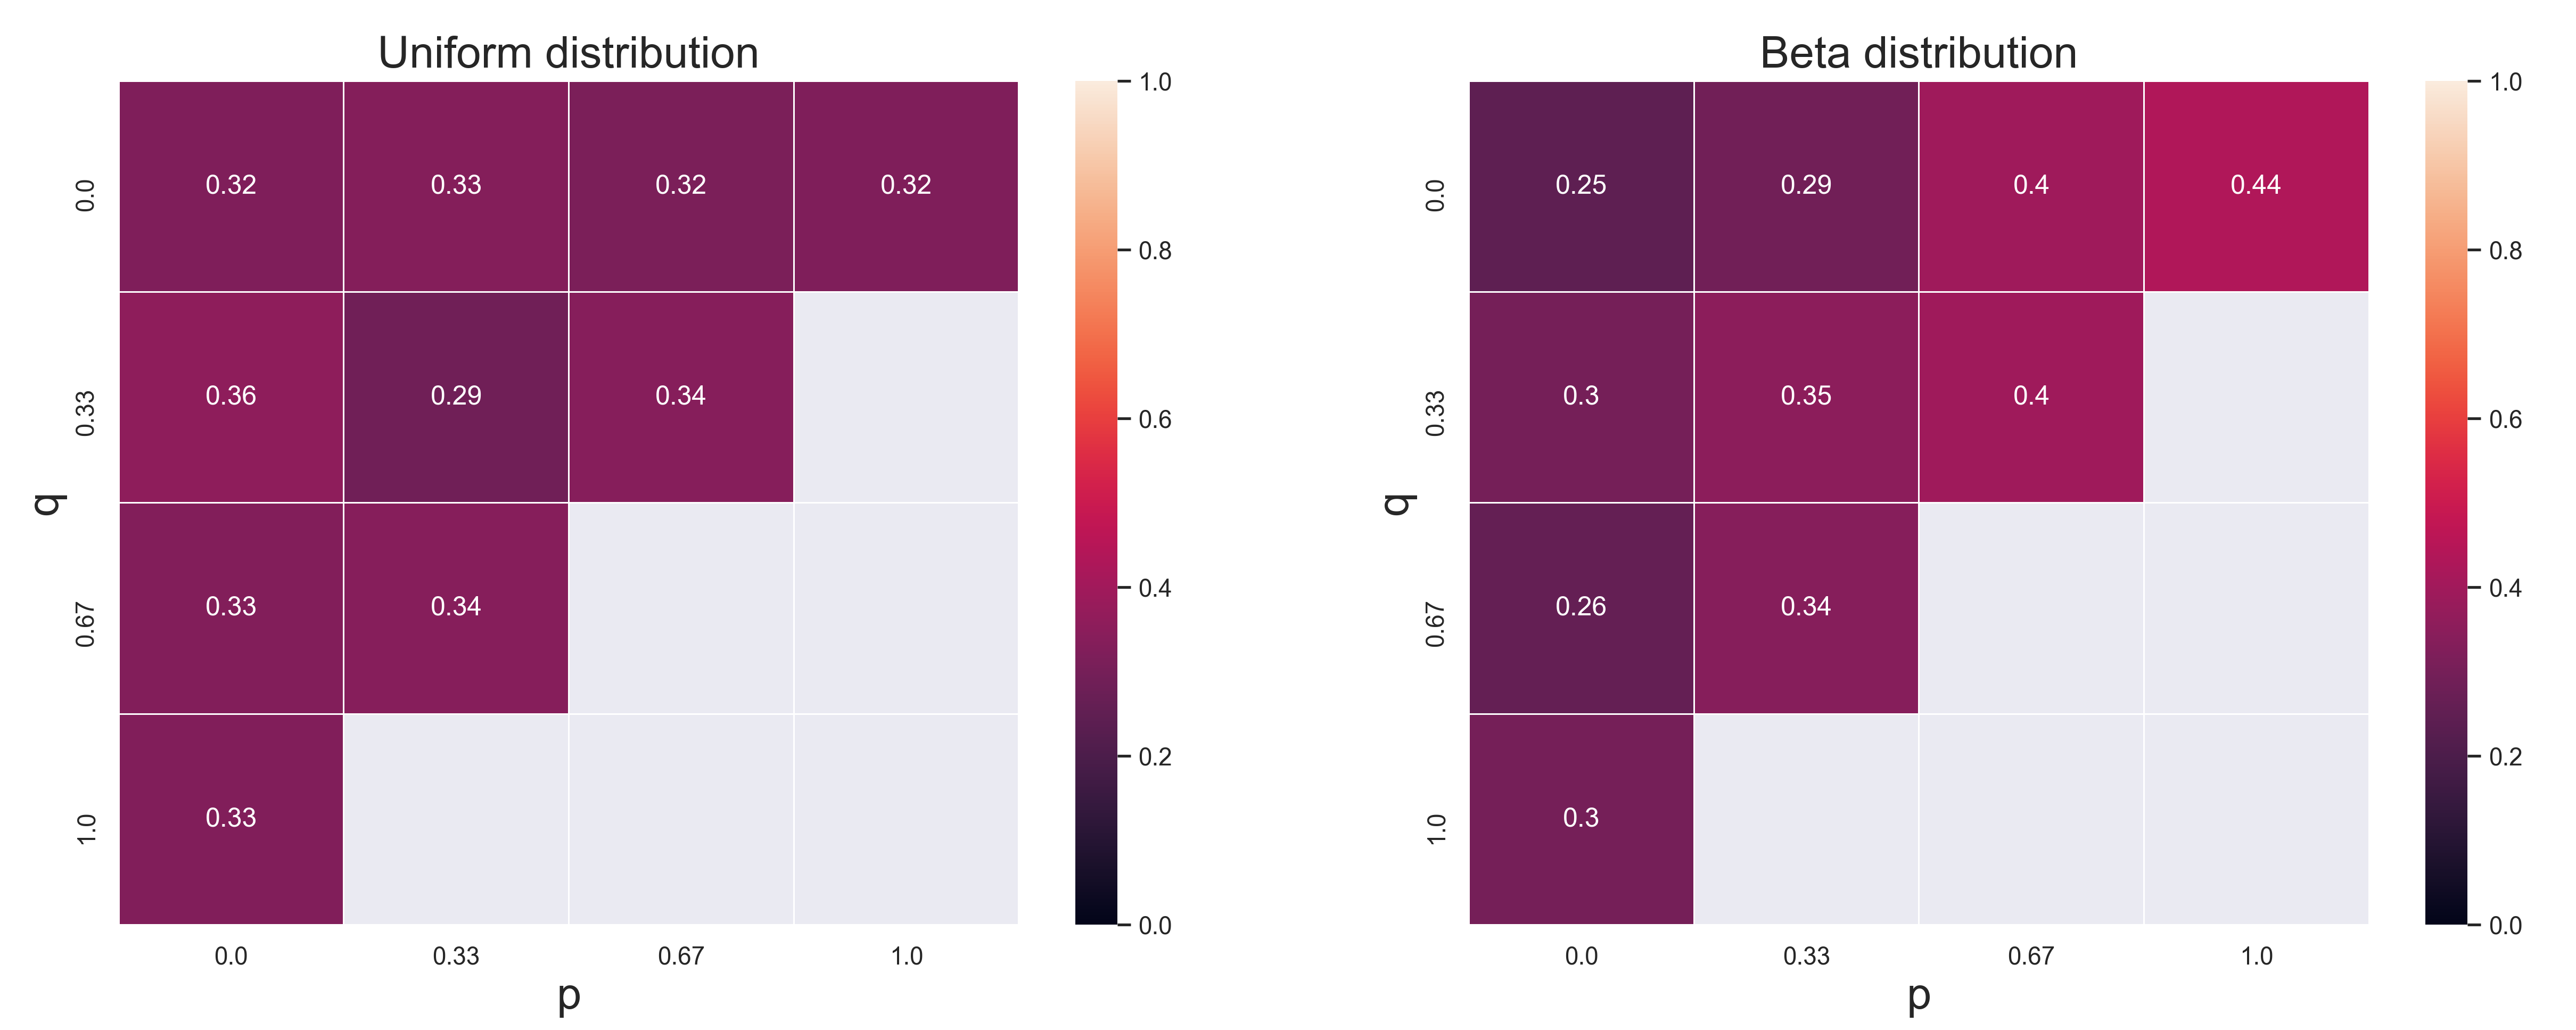
\includegraphics[scale=0.4]{"Images/Task1.png"}


\section{Task 2}
\subsection{Theoretical solution}
\subsubsection{Problem 1}
Consider $X_1, \ldots X_n$ --- i.i.d such that $X_i \sim U[0, 1], \forall i = 1, \ldots, n.$
As we know
$$
\mathbb{E} X_{(r)} = \int \limits_{-\infty}^{+\infty} x d F_{X_{(r)}}(x),
$$
where $F_{X_{(r)}}(x)$ is CDF of $X_{(r)}.$

\begin{theorem}
Let $F_X(x)$ be the common CDF of the r.v. $X.$ For $r = 1, \ldots, n,$
$$
F_{X_{(r)}}(x) = \mathbb{P} (X_{(k)} \leqslant x) = \sum \limits_{k = r}^n C_n^k (F_X (x))^k (1 - F_X (x) )^{n - k}.
$$
\end{theorem}
\begin{proof}
Note, that in a sample $\{X_1, \ldots, X_n\}$ of $n$ independent values the number of observations not bigger than $x$ has $Bin(n, F_X(x))$ distribution.
By breaking the event $\{X_{(r)} \leqslant x\}$ into simple disjoint events, we get
$$
\{X(r) \leqslant x\} = A_n(x) \bigcup \ldots \bigcup A_r(x) = 
$$
$$
 = \{X_{(n)} \leqslant x\} \bigcup \{X_{(n-1)} \leqslant x, X_{(n)} > x\}  \bigcup
$$
$$
\ldots
$$
$$
\bigcup \{X_{(r)} \leqslant x, X_{(n)} > x, \ldots X_{(r - 1)} > x\}.
$$
Then 
$$
F_{X_{(r)}}(x) = \P ( X_{(r)}  \leqslant x ) = \P \left(\mathop{\bigcup} \limits_{k = r}^n  A_k(x) \right) = \sum \limits_{k=r}^n \P(A_k(x)) = 
$$
$$ = \sum \limits_{k = r}^n C_n^k (F_X (x))^k (1 - F_X (x) )^{n - k}.
$$
\end{proof}
\noindent We also know that
$$
\dfrac{d F_X(x)}{dx} = f_X(x),
$$
where $f_X(x)$ is density function of $X.$ 
If $X \sim U[0, 1],$ then we derive the next equation
$$
\dfrac{d F_{X_{(r)}}(x)}{dx} = \sum \limits_{k = r}^n C_n^k [k x^{k-1} (1 - x )^{n - k} - (n - k) x^k (1 - x)^{n - k - 1}] = f_{X_{(r)}}(x).
$$
Finally, we have
$$
\E X_{(r)} = \int \limits_{-\infty}^{+\infty} x f_{X_{(r)}}(x) dx = 
$$
$$
= \sum \limits_{k = r}^n k C_n^k  \int \limits_{0}^{1} [x^k (1 - x )^{n - k}] dx - \sum \limits_{k = r}^n (n - k) C_n^k  \int \limits_{0}^{1} [x^{k+1} (1 - x)^{n - k - 1}] dx = 
$$
$$
= \sum \limits_{k = r}^n k C_n^k  B(k+1, n-k+1) - \sum \limits_{k = r}^n (n - k) C_n^k B(k + 2, n - k) = 
$$
$$
= \sum \limits_{k = r}^n \dfrac{k \cdot n!}{(n-k)! k!}  \dfrac{k! (n-k)!}{(n + 1)!} - \sum \limits_{k = r}^n  \dfrac{(n - k) \cdot n!}{(n-k)! k!}  \dfrac{(k + 1)! (n-k-1)!}{(n+ 1)!} = 
$$
$$
= \dfrac{r}{n+1}.
$$
\subsubsection{Problem 2}
We derive the next equation using the result from \textbf{Problem 1}:
$$
\E X_{(r)}^2 = \int \limits_{-\infty}^{+\infty} x^2 f_{X_{(r)}}(x) dx = 
$$
$$
= \sum \limits_{k = r}^n k C_n^k  \int \limits_{0}^{1} [x^{k+1} (1 - x )^{n - k}] dx - \sum \limits_{k = r}^n (n - k) C_n^k  \int \limits_{0}^{1} [x^{k+2} (1 - x)^{n - k - 1}] dx = 
$$
$$
= \sum \limits_{k = r}^n k C_n^k  B(k+2, n-k+1) - \sum \limits_{k = r}^n (n - k) C_n^k B(k + 3, n - k) = 
$$
$$
= \sum \limits_{k = r}^n \dfrac{k \cdot n!}{(n-k)! k!}  \dfrac{(k+1)! (n-k)!}{(n + 2)!} - \sum \limits_{k = r}^n  \dfrac{(n - k) \cdot n!}{(n-k)! k!}  \dfrac{(k + 2)! (n-k-1)!}{(n+ 2)!} = 
$$
$$
= \dfrac{r (r+1)}{(n+1)(n+2)}.
$$
\subsubsection{Problem 3}
Transform the next equation 
$$
f_{X_{(r)}}(x) = \sum \limits_{k = r}^n C_n^k [k x^{k-1} (1 - x )^{n - k} - (n - k) x^k (1 - x)^{n - k - 1}] = 
$$
$$
= C_n^{k-1} x^{r-1} (1 - x)^{n-r} + \sum \limits_{k = r+1}^n C_n^k [k x^{k-1} (1 - x )^{n - k}] - \sum \limits_{k = r}^{n-1} C_n^k [(n - k) x^k (1 - x)^{n - k - 1}].
$$
The last two terms above cancel, since using the change of variables $j = k - 1.$
Now we can find the maximum of $f_{X_{(r)}}(x):$
$$
\dfrac{d f_{X_{(r)}}(x)}{d x} = C_n^{k-1} [(r-1)x^{r-2} (1 - x)^{n-r} - (n - r)x^{r-1}(1-x)^{n-r-1}] = 0.
$$
The solutions of this equation are
$$
x = 0, x = 1, x = \dfrac{r-1}{n-1},
$$
but the maximum of $f_{X_{(r)}}(x)$ is attained on $x = \dfrac{r-1}{n-1}.$
\subsection{Numerical solution}
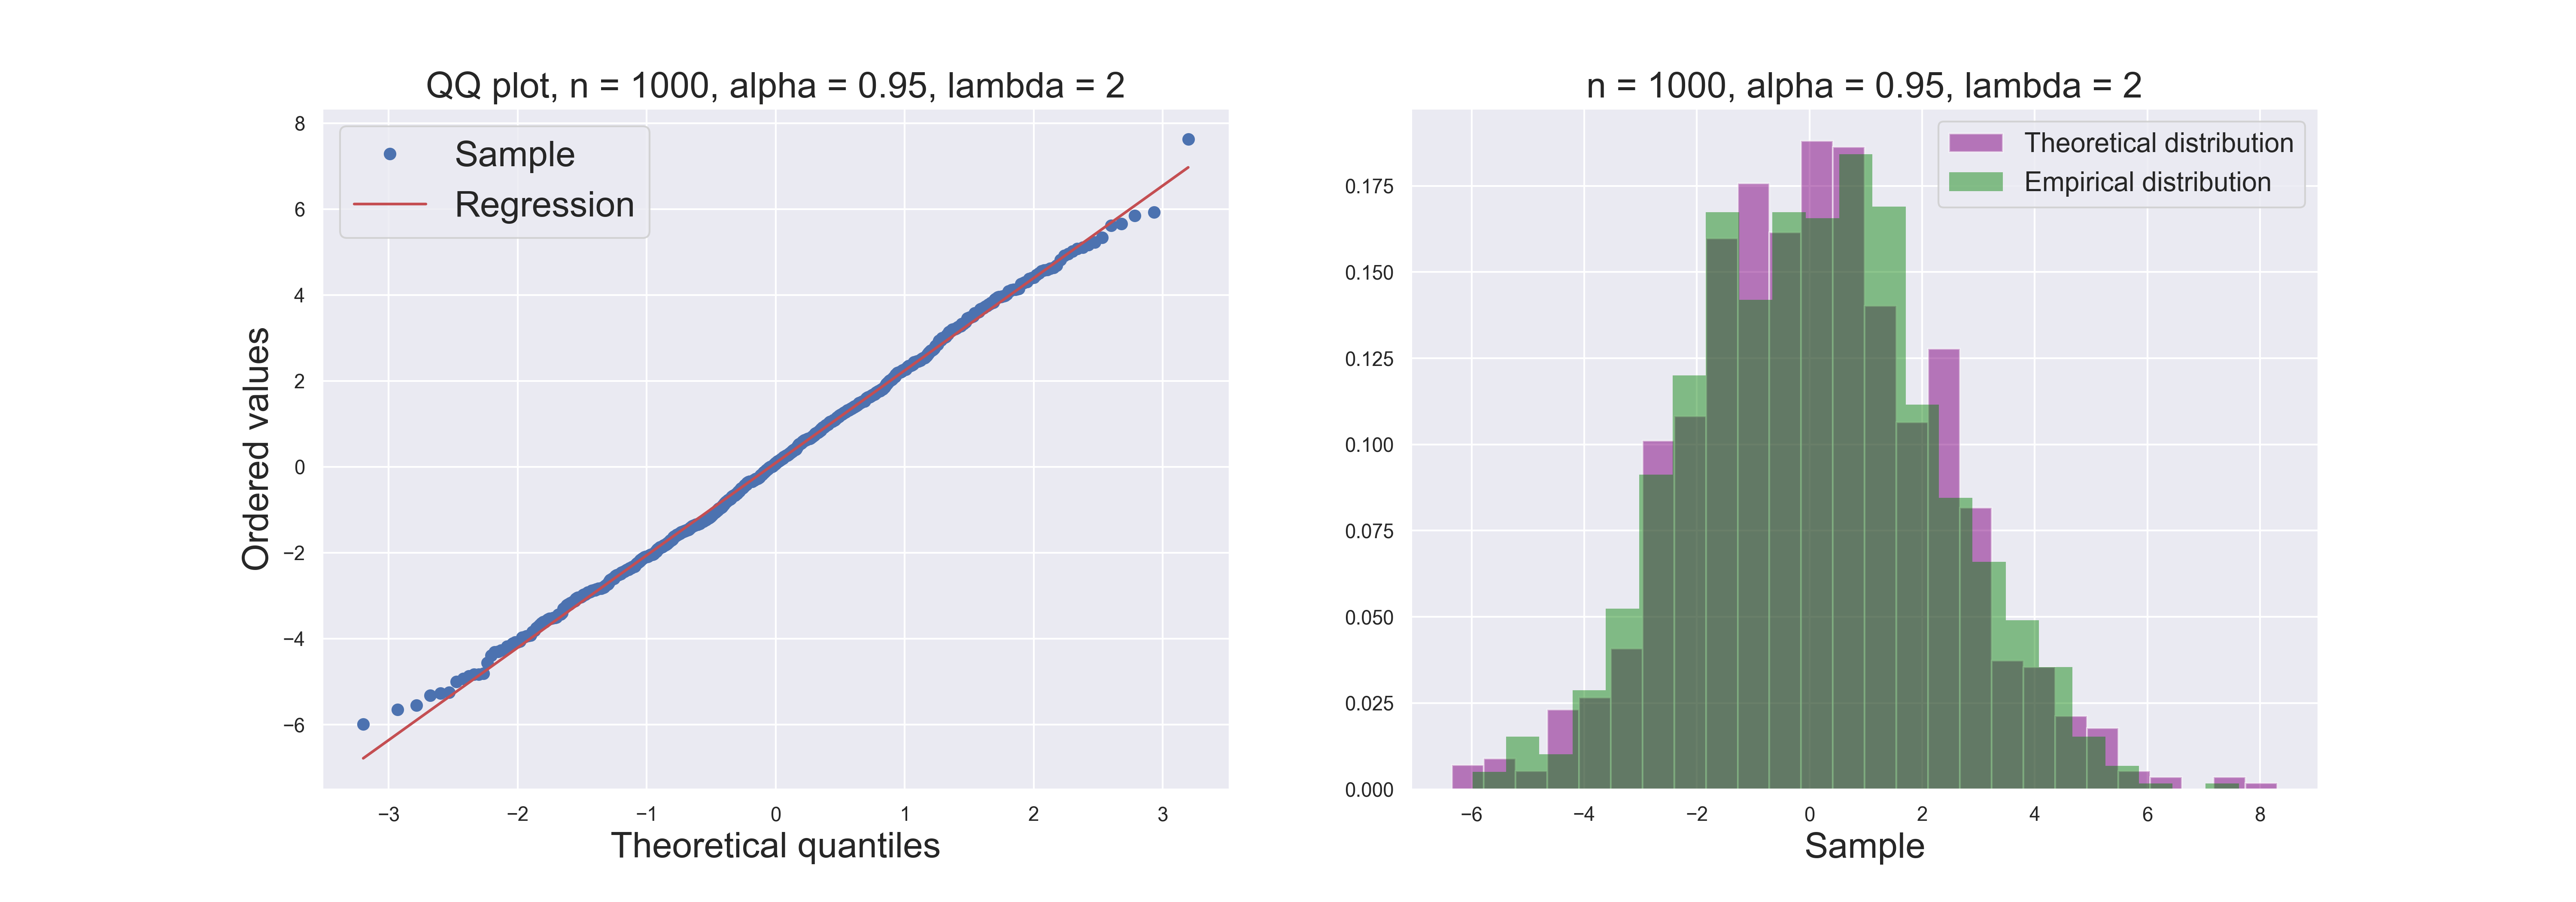
\includegraphics[width=\textwidth]{"Images/Task2_1000.png"}
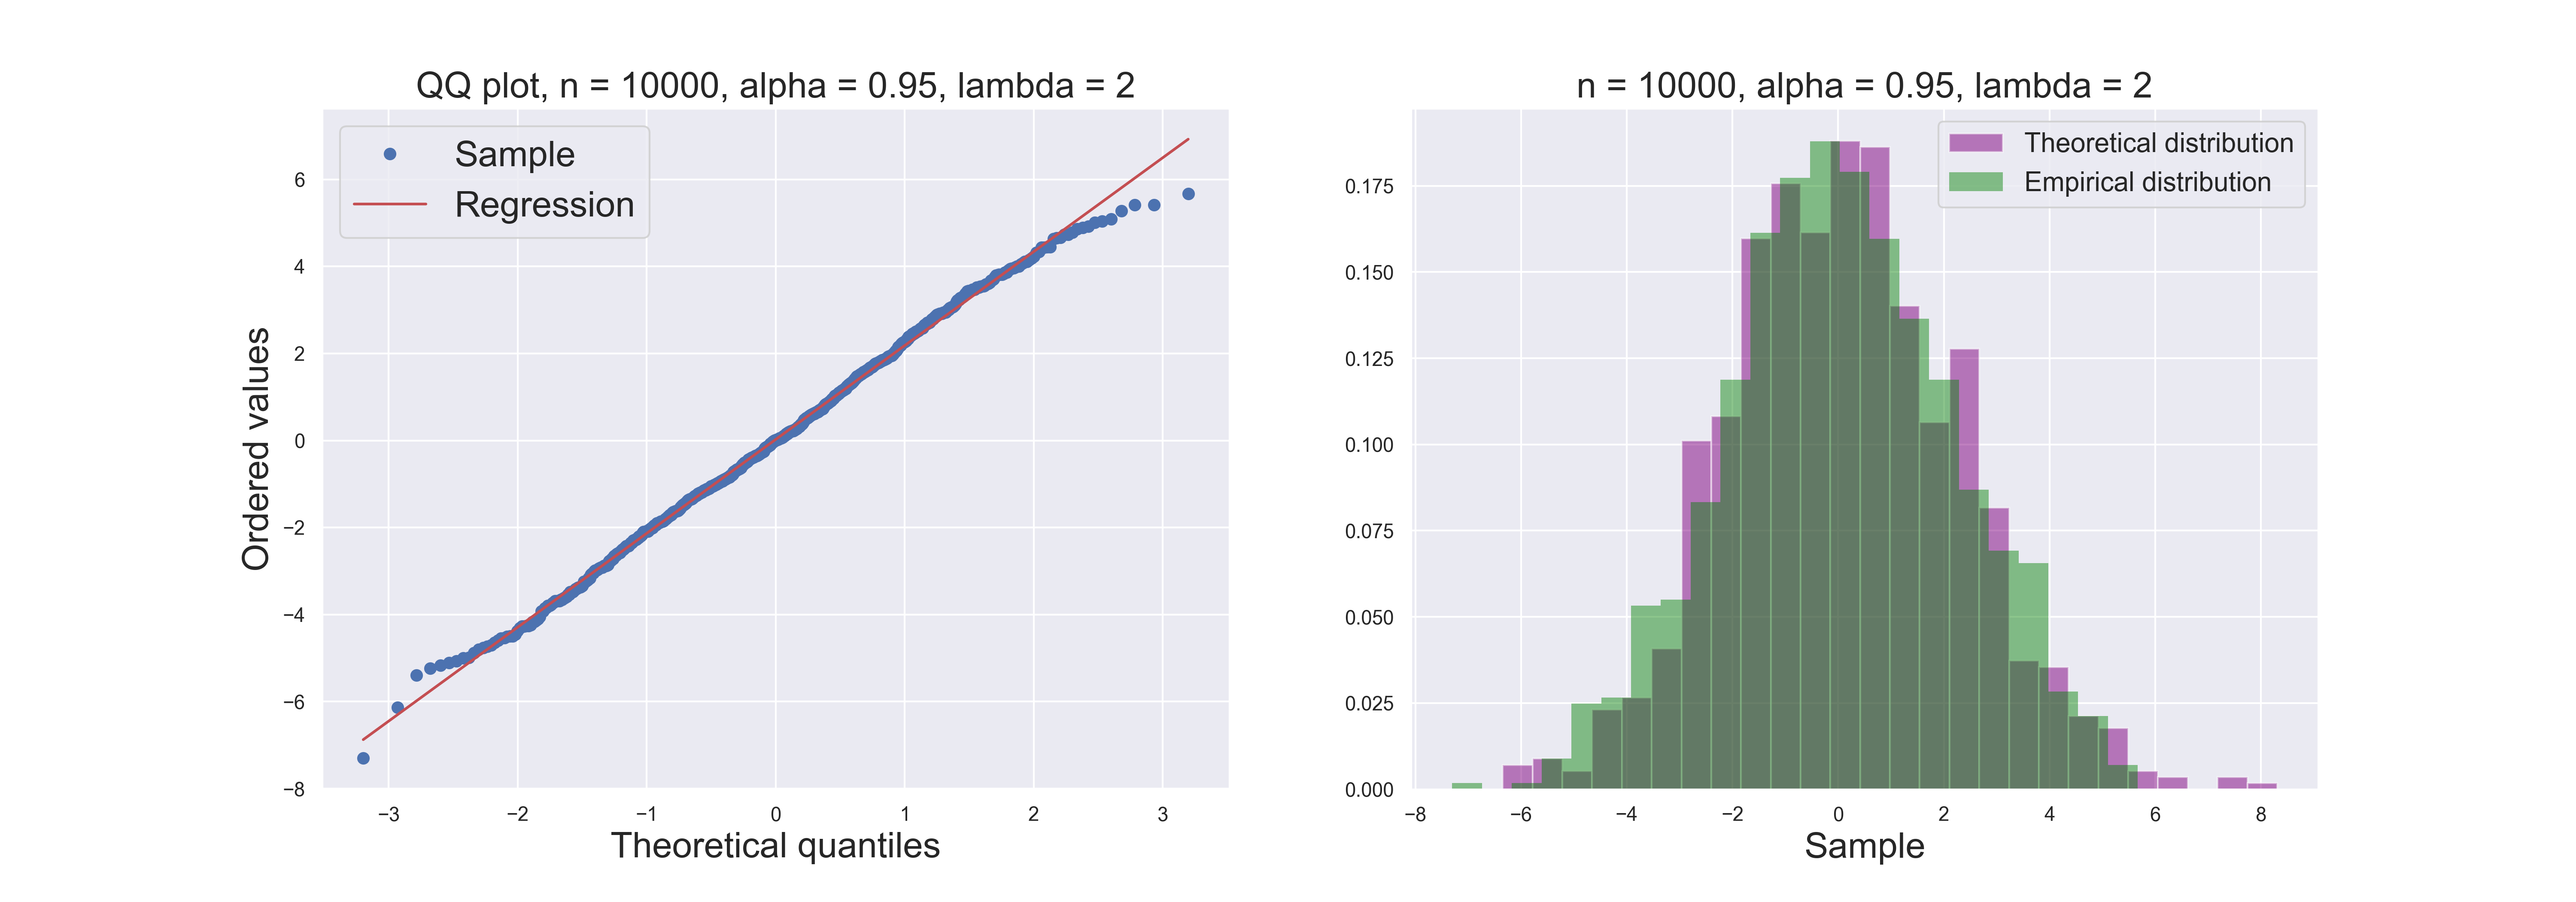
\includegraphics[width=\textwidth]{"Images/Task2_10000.png"}
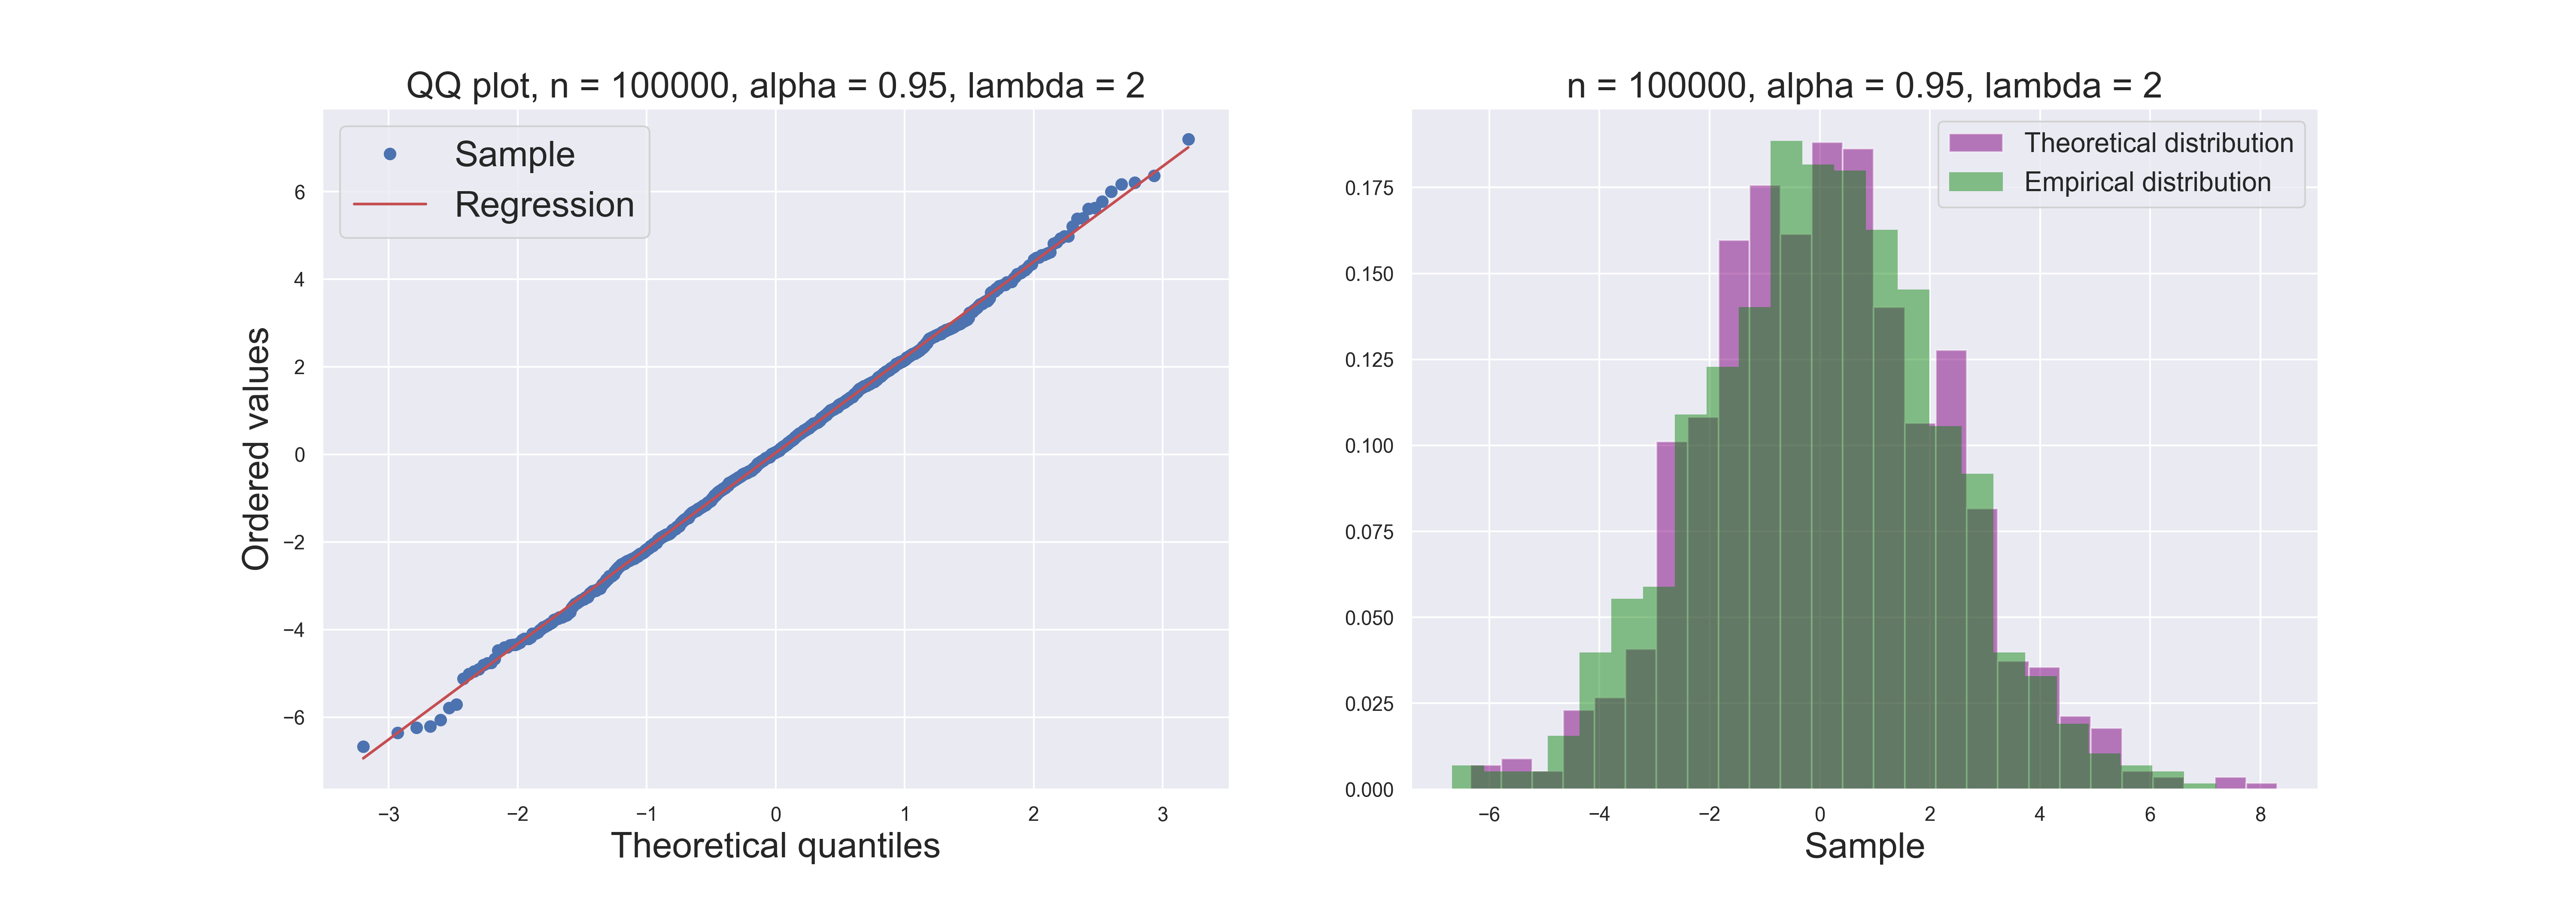
\includegraphics[width=\textwidth]{"Images/Task2_100000.png"}

\section{Task 3}
\subsection{Theoretical solution}
\subsubsection{Problem 1 (MLE method)}
Let $X_1, \ldots, X_n$ be a sequence of i.i.d random variables.
Consider log-likelihood function 
$$
l(\mu, \sigma) = \log p(x_1, \ldots, x_n; \mu, \sigma) = \sum \limits_{i=1}^n \log p(x_i; \mu, \sigma) \rightarrow \max \limits_{\mu, \sigma}.
$$
\begin{itemize}
	\item We find the next estimation $\hat{\sigma}_n$ as follows:
$$
\dfrac{dl(\mu, \sigma)}{d \mu} = \sum \limits_{i=1}^n \left[ - \dfrac{1}{\sigma} + \dfrac{|x_i - \mu|}{\sigma^2} \right] = 0,
$$
$$
\hat{\sigma}_n = \dfrac{1}{n} \sum \limits_{i=1}^n |x_i - \mu|.
$$
	\item We find the next estimation $\hat{\mu}_n$ as follows. The likelihood function 
$$
\mathcal{L}(\mu, \sigma) = \dfrac{1}{(2 \sigma)^n} \exp \left(- \dfrac{1}{\sigma} \sum \limits_{i=1}^n |x_i - \mu| \right)
$$
is supposed to be maximized $\Leftrightarrow$ when $ \sum \limits_{i=1}^n |x_i - \mu|$ is supposed to be minimized.
\begin{theorem}
Let $m$ be the sample median, then then next inequality 
$$
 \sum \limits_{i=1}^n |x_i - \mu| \geqslant  \sum \limits_{i=1}^n |x_i - m|
$$
holds for every value of $\mu$
\end{theorem}
\begin{proof}
Consider  two cases.
\begin{enumerate}
	\item Let $n$ be even. Let $m$ be any real number between the two middle values so that we have
$$
x_{(1)} \leqslant \ldots \leqslant x_{(\frac{n}{2})} \leqslant \mu \leqslant x_{(\frac{n}{2} + 1)} \leqslant \ldots \leqslant x_{(n)}.
$$
For $\left \{i = 1, \ldots, \dfrac{n}{2} \right \}$ the triangle inequality gives us
$$
|x_{(i)} - m| + |m - x_{(n - i + 1)}| = |x_{(n - i + 1)} - x_{(i)}|  \leqslant |x_{(i)} - \mu| + |\mu - x_{(n - i + 1)}|.
$$
Hence,
$$
\sum \limits_{i=1}^{\frac{n}{2}} |x_{(i)} - m| + |m - x_{(n - i + 1)}| \leqslant \sum \limits_{i=1}^{\frac{n}{2}} |x_{(i)} - \mu| + |\mu - x_{(n - i + 1)}|
$$
and
$$
\sum \limits_{i=1}^{\frac{n}{2}} |m - x_{(n - i + 1)}| = \sum \limits_{i=\frac{n}{2}+1}^n |m - x_{(i)}|,
$$
$$
\sum \limits_{i=1}^{\frac{n}{2}} |\mu - x_{(n - i + 1)}| = \sum \limits_{i=\frac{n}{2}+1}^n |\mu - x_{(i)}|. 
$$
As a result we have
$$
\sum \limits_{i=1}^n |m - x_{(i)}| \leqslant \sum \limits_{i=1}^n |\mu - x_{(i)}|.
$$
	\item  Let $n$ be odd. Then $m = x_{(\frac{n + 1}{2})}$ is the sample median:
$$
x_{(1)} \leqslant \ldots \leqslant x_{(\frac{n+1}{2})}  \leqslant \ldots \leqslant x_{(n)}.
$$
For $i = \left \{ 1, \ldots, \dfrac{n + 1}{2} \right\}$ the triangle inequality gives us
$$
|x_{(i)} - x_{(\frac{n + 1}{2})}| + |x_{(\frac{n + 1}{2})} - x_{(n - i + 1)}| = |x_{(n - i + 1)} - x_{(i)}|  \leqslant |x_{(i)} - \mu| + |\mu - x_{(n - i + 1)}|.
$$
Hence,
$$
\sum \limits_{i=1}^{\frac{n+1}{2}} |x_{(i)} - x_{(\frac{n + 1}{2})}| + |x_{(\frac{n + 1}{2})} - x_{(n - i + 1)}| \leqslant \sum \limits_{i=1}^{\frac{n+1}{2}} |x_{(i)} - \mu| + |\mu - x_{(n - i + 1)}|
$$
and
$$
\sum \limits_{i=1}^{\frac{n+1}{2}} |x_{(\frac{n + 1}{2})} - x_{(n - i + 1)}| = \sum \limits_{i=\frac{n+1}{2}}^n |x_{(\frac{n + 1}{2})}- x_{(i)}|,
$$
$$
\sum \limits_{i=1}^{\frac{n+1}{2}} |\mu - x_{(n - i + 1)}| = \sum \limits_{i=\frac{n+1}{2}}^n |\mu - x_{(i)}|. 
$$
As a result we have
$$
\sum \limits_{i=1}^n |x_{(\frac{n + 1}{2})} - x_{(i)}| \leqslant \sum \limits_{i=1}^n |\mu - x_{(i)}|.
$$	
\end{enumerate}
\end{proof}
The estimation parameters are  
$$
\hat{\mu}_n = median \{x_1, \ldots, x_n \}, 
$$
$$
\hat{\sigma}_n = \dfrac{1}{n} \sum \limits_{i=1}^n |x_i - \hat{\mu}_n|.
$$
\end{itemize}
\subsubsection{Problem 2 (Method of moments)}
Consider $X_1, \ldots, X_n$ --- i.i.d such that $X_i \sim Laplace(\mu, \sigma), \forall i = 1, \ldots, n.$ Then we need to solve the next system
$$
\begin{cases}
\mu = \dfrac{1}{n} \sum \limits_{i=1}^n x_i, \\
\mu^2 + 2 \sigma^2 = \dfrac{1}{n} \sum \limits_{i=1}^n x_i^2,
\end{cases}
$$
from which we derive that
$$
\hat{\mu}_n = \dfrac{1}{n} \sum \limits_{i=1}^n x_i, 
$$
$$
\hat{\sigma}_n = \sqrt{\dfrac{1}{2n} \sum \limits_{i=1}^n x_i^2 - \dfrac{1}{2} \left( \dfrac{1}{n} \sum \limits_{i=1}^n x_i \right)^2 }.
$$
\subsection{Numerical solution}
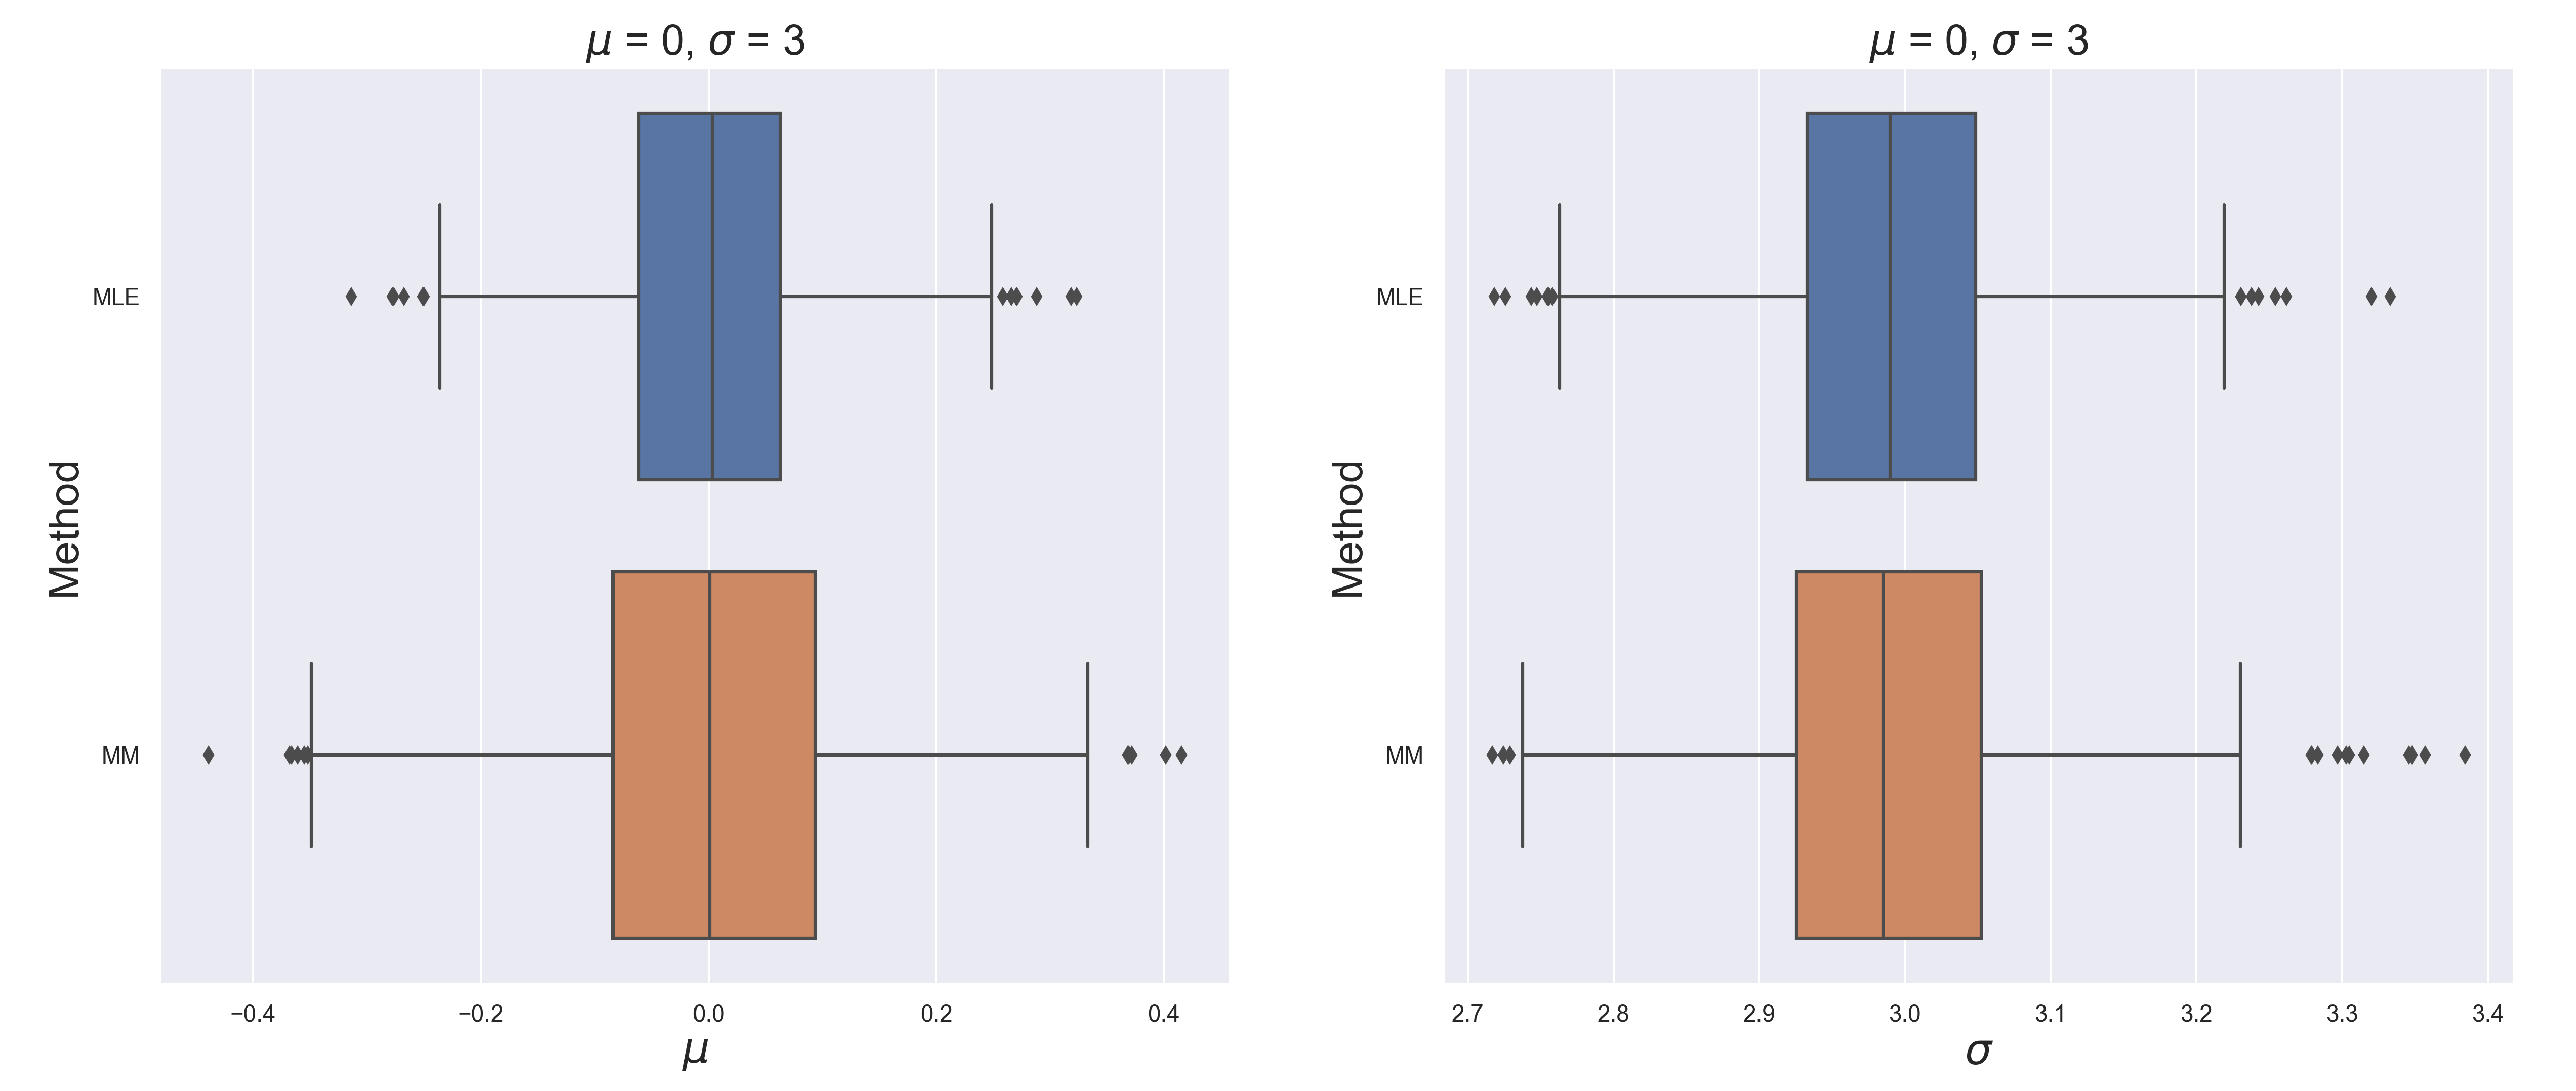
\includegraphics[width=\textwidth]{Images/Task3.png}
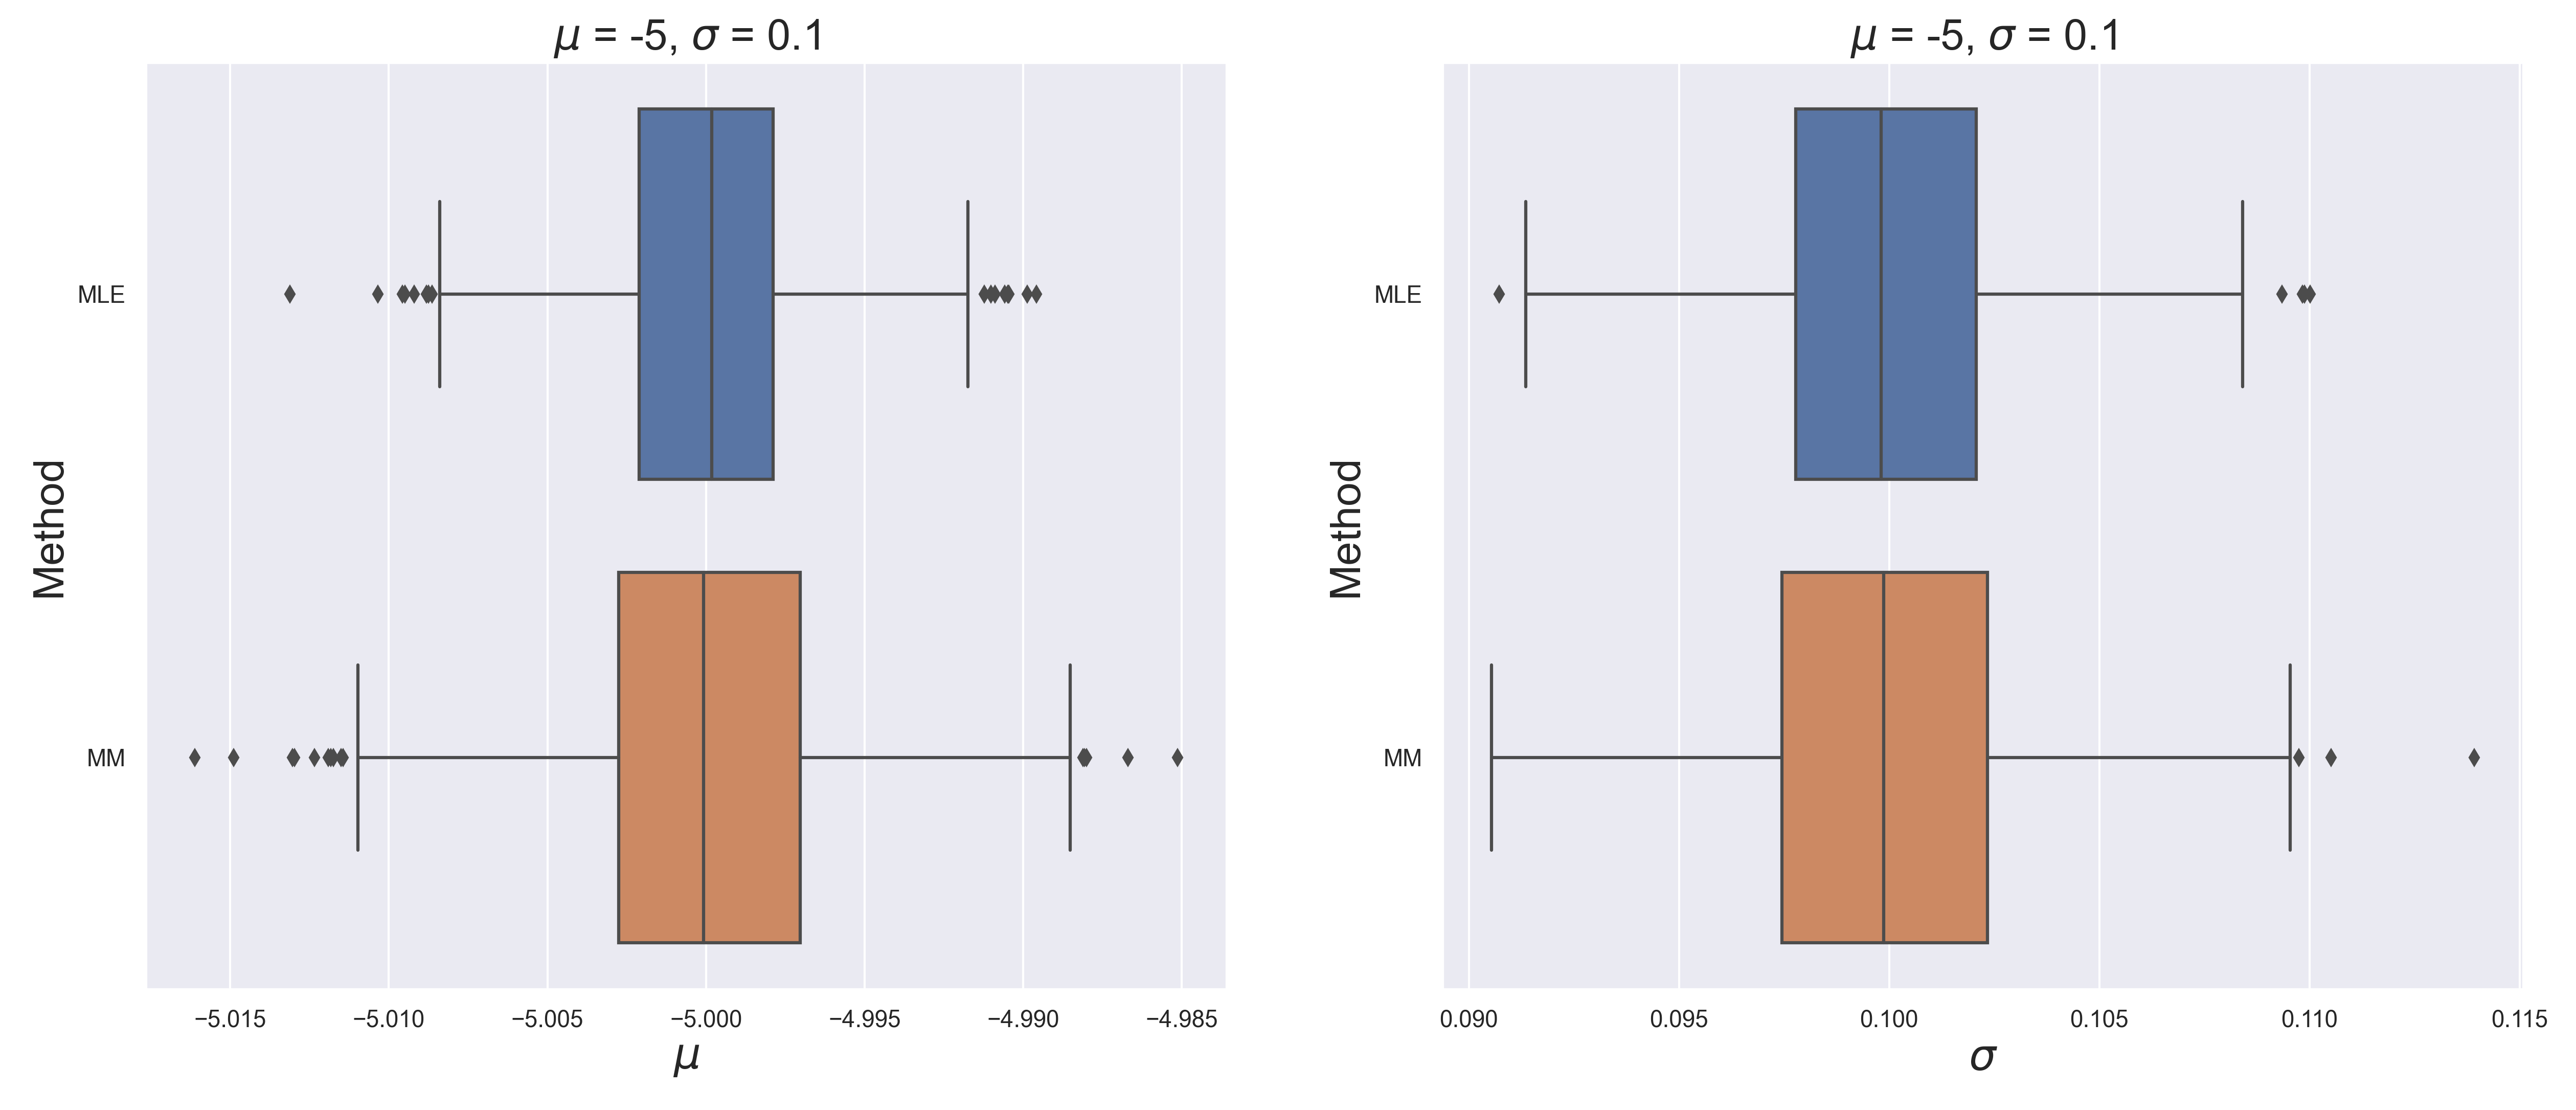
\includegraphics[width=\textwidth]{Images/Task3_1.png}
We can see that MLE method is better a little bit than MM method.


\section{Task 4}
\subsection{Theoretical solution}
\subsubsection{Problem 1}
Let's calculate the density function of $\xi^2$ as $f_{\xi^2}(x) = \dfrac{dF_{\xi^2}(x)}{dx}.$ Firstly,
$$
F_{\xi^2}(x) = \P(\xi^2 \leqslant x) =  \P(|\xi | \leqslant \sqrt{x}) = \int \limits_{-\sqrt{x}}^{\sqrt{x}} f_{\xi}(t) dt = 
$$
$$
f_{\xi^2}(x) = \dfrac{f_{\xi}(\sqrt{x}) + f_{\xi}(-\sqrt{x})}{2 \sqrt{x}} = \{ \xi \sim \mathcal{N}(0, \theta)\} = \dfrac{f_{\xi}(\sqrt{x})}{\sqrt{x}}.
$$
Now we can decompose the density function $f_{\xi^2}(x)$ as follows:
$$
f_{\xi^2}(x) = \dfrac{1}{\sqrt{x}} \dfrac{1}{\sqrt{2 \pi  \theta}} \exp \left( -\dfrac{x}{2 \theta} \right) = h(x) \cdot \exp \left(v x - g(v)) \right)
$$
where
$$
h(x) = \dfrac{1}{\sqrt{2 \pi x}},
$$
$$
v = -\dfrac{1}{2  \theta},
$$
$$
g(v) = \log \left (\sqrt{-\dfrac{1}{2v}} \right) = -\dfrac{1}{2} \log (-2v).
$$
Thus, $P_{\sigma^2} = \{Law(\xi^2), ~ \xi \sim \mathcal{N}(0, \theta) \}$ is an exponential family.
\subsubsection{Problem 2}
Consider $X \sim P_{\theta}.$ Simple derivation gives us
$$
\E [X] = g^{\prime} (v) = -\dfrac{1}{2  v} = \theta,
$$
$$
\Var [X] = g^{\prime \prime} (v) = \dfrac{1}{2 v^2} = 2 \theta^2.
$$ 
\paragraph{MLE method.} Construct the log-likelihood function
$$
l(\theta) = \log p(x_1, \ldots, x_n; \theta) =  \sum \limits_{i=1}^n \log p(x_i; \theta)
$$
which is supposed to be maximized by $\theta.$
Using optimality condition we get
$$
\sum \limits_{i=1}^n \dfrac{d}{d\theta} \left[-\dfrac{1}{2}\log (2 \pi x_i) - \dfrac{1}{2} \log (\theta) - \dfrac{x_i}{2\theta} \right]  = 0,
$$
$$
\hat{\theta}_n = \dfrac{1}{n} \sum \limits_{i=1}^n x_i.
$$

\paragraph{Method of moments.} Using the result above we derive the first moment
$$
\theta =  \dfrac{1}{n} \sum \limits_{i=1}^n x_i,
$$
from which we get
$$
\hat{\theta}_n = \dfrac{1}{n} \sum \limits_{i=1}^n x_i.
$$

\subsection{Numerical solutions}
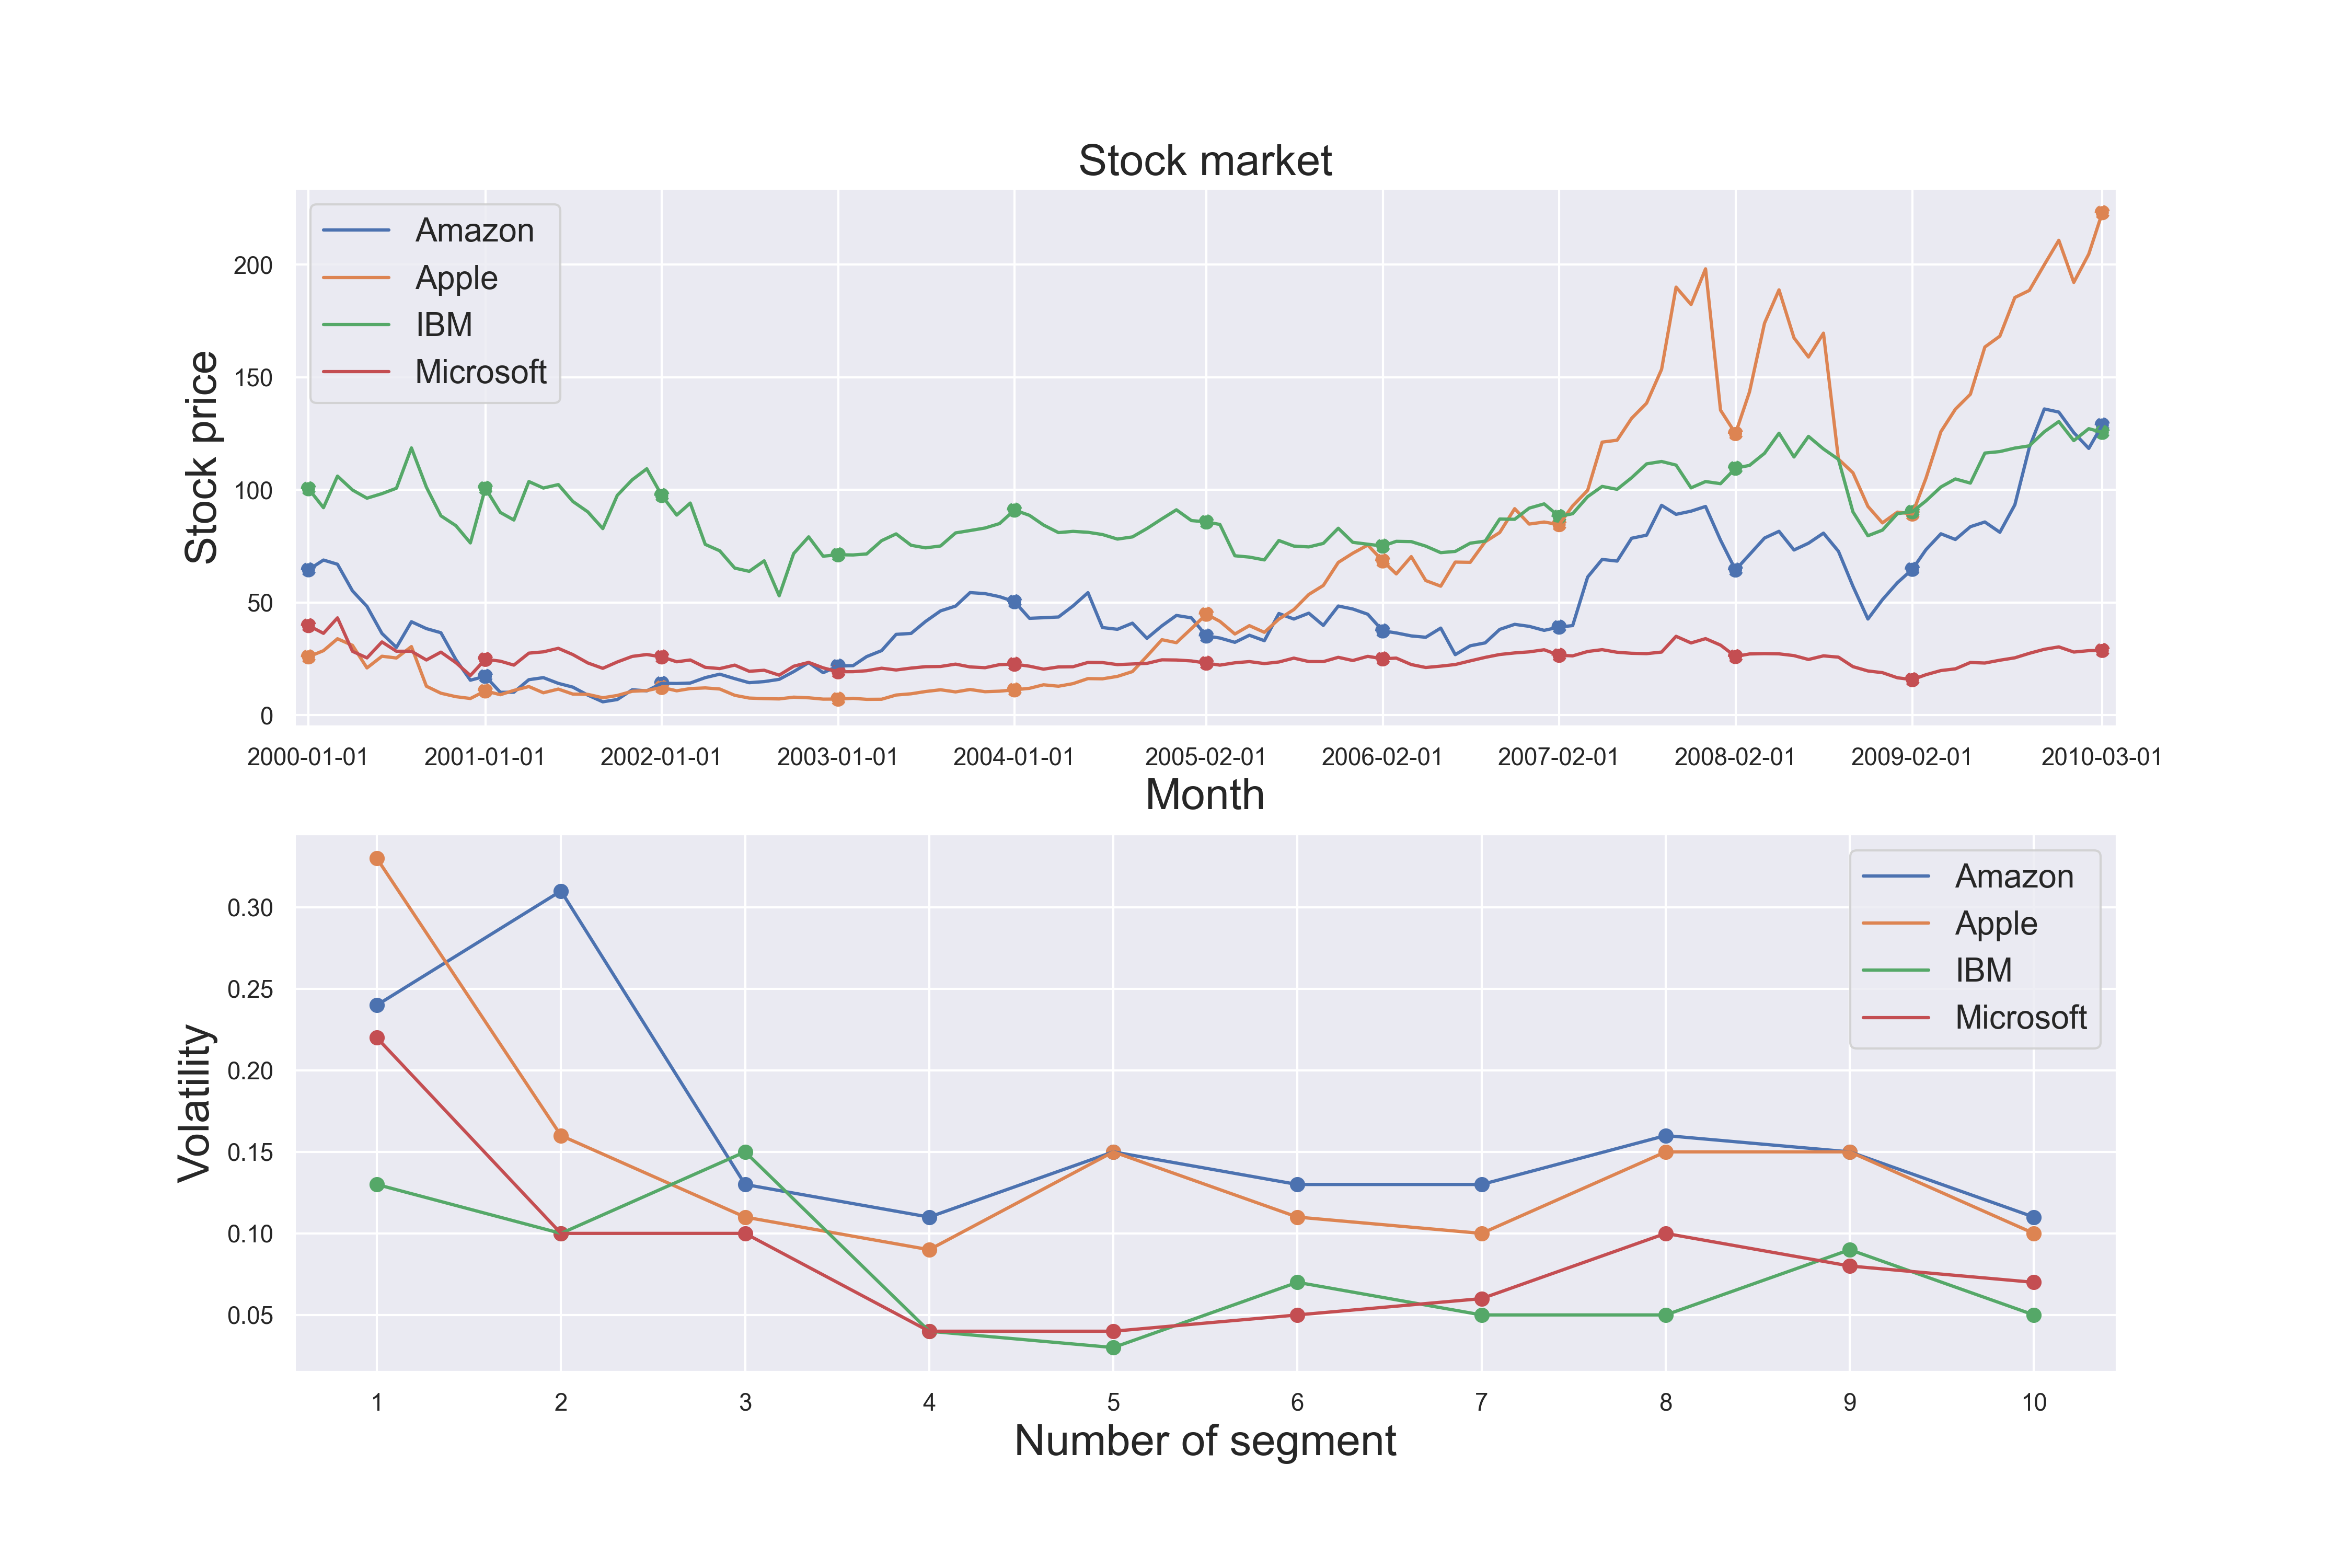
\includegraphics[width=\textwidth]{Images/Task4.png}
We split the top graph with points and now we have 10 time segments. Each point on bottom graph represents volatility parameter on corresponding interval. As we can see the volatility of Amazon and Apple companies higher than  the volatility of IBM and Microsoft.

\section{Appendix}
\begin{itemize}
	\item Code can be found: \href{https://github.com/vitomania/ozon/blob/master/stats/hw1/Numerical_solution.ipynb}{here};
	\item The data for \textbf{Task 4} was taken from \href{https://github.com/vega/datalib/blob/master/test/data/stocks.csv}{here}.
\end{itemize}
\end{document} 